\chapter{Resultados Experimentais} \label{exp}

%Este capítulo apresenta os resultados dos experimentos feitos para validar o método de detecção e extração do conteúdo de telas de TV e monitores. Eles foram implementados na linguagem MATLAB, na versão R2012a, em ambiente Linux, processador Intel(R) Core(TM) i7-3770 CPU @ 3.40GHz e memória RAM 16GB.

Para validar o método de detecção e extração do conteúdo de telas de TV e monitores, desenvolvido no Capítulo \ref{met}, foram feitos experimentos que abordam o problema da inspeção automática de TVs e monitores. 

%falar um pouco mais sobre inspeção automática de monitores. aquela referencia do Kastelan. procurar mais

%Com o volume de produção de eletrônicos de consumo, tem se mostrado necessário o uso de sistemas de inspeção automática para verificar a qualidade do produto ou de partes dele conforme vão sendo produzidos. Este tipo de inspeção tem ganhado terreno em relação à inspeção manual devido à maior precisão,  menor tempo de inspeção e uso de recursos humanos \cite{vantagemauto}.

%Muitos sistemas de inspeção automática de telas de TV e monitores têm sido propostos \cite{vantagemauto,sistauto00,sisauto01,sisauto02}. Entretanto, a abordagem adotada por este método, de comparar imagens de referência com fotos do monitor, têm ainda poucos trabalhos \cite{inspect}.

Neste capítulo serão apresentados os resultados experimentais obtidos nas simulações feitas, assim como detalhará os experimentos. O capítulo será organizado como segue: na primeira seção, mostramos o \textit{setup} dos experimentos, seguida por uma seção que detalha as bases de dados utilizadas. A terceira seção explica as métricas de desempenho de cada experimento, finalizando o capítulo com uma seção detalhando os procedimentos experimentais e a última seção expondo e analisando os resultados.
%o que pode ser inspecionado? que erros são comuns? um paragrafo

%breve resumo do que sera encarado nas próximas seções
%três experimentos foram executados. O primeiro visa comparar o custo em tempo do método original e o método proposto, que utiliza redimensionamento das imagens. O segundo experimento submete ao método as 504 imagens da primeira base de dados e as 600 da segunda, visando verificar a capacidade de corretamente relacionar a tela encontrada com uma imagem de referência. O terceiro experimento visa submeter as mesmas imagens ao método com as modificações propostas, afim de comparar os resultados alcançados com os do método original.

%A base de dados um consiste em um conjunto de 504 fotos coloridas de monitores e telas de TV, em três tamanhos diferentes e condições não controladas de iluminação e captura, assim como seis imagens de referência de resolução 1600 por 900 pixeis. Cada foto é acompanhada por uma marcação de coordenadas que indicam os quatro vértices da tela na foto. Eles são tidos como \textit{ground truth}.

\section{Setup dos Experimentos}

Os experimentos foram implementados na linguagem MATLAB, na versão R2012a, em ambiente Linux, processador Intel(R) Core(TM) i7-3770 CPU @ 3.40GHz e memória RAM 16GB. Para fins de simulação, o cálculo da transformada de Hough foi feito utilizando a própria função interna do Matlab. Diversos \textit{scripts} foram programados e combinados para que fosse possível implementar as simulações propostas, assim como para a geração dos rótulos com as coordenadas da tela nas fotos. As imagens de treino e de teste foram capturadas, armazenadas e usadas como entrada dos \textit{scripts}.

%Todas as imagens de base têm formato RGB.

\section{Bases de Dados}

%Após extensiva pesquisa em bancos de imagens, não foi encontrada uma base de dados que atenda aos interesses deste trabalho.

%citar bases pesquisadas

% o que foi procurado
Para os experimentos, se fez necessário um conjunto de imagens em par, em que cada par era composto por:
\begin{itemize}
\item a foto de um monitor ou televisão ligado com conteúdo sendo mostrado;
\item uma cópia do conteúdo mostrado na tela ou monitor, para fins de comparação;
\end{itemize}

Após extensiva pesquisa em bancos de imagens, não foi encontrada uma base que tivesse conteúdo semelhante. Portanto, se fez necessário montar uma base própria. Foram feitas duas, uma com 6 imagens de referência e 504 imagens de teste em um ambiente não controlado, outra com 40 imagens de referência e 600 imagens de teste em um ambiente controlado.

\subsection{Primeira Base}

%As imagens de referência da primeira base foram escolhidas entre menus e vídeos da internet. Quatro seleções diferentes de um menu foram utilizadas, assim como dois frames de um vídeo. As imagens são coloridas e têm resolução 1600 x 900 pixeis. As fotos dos 14 monitores foram feitas com os mesmos ligados e mostrando cada uma das seis imagens. A câmera utilizada foi a câmera do celular Samsung Galaxy S5, com sensor de 16 MP, abertura de 2,2 polegadas, foco automático e sem flash. As fotos foram feitas utilizando os tamanhos 5312 x 2988 pixeis, [resolução 2] e [resolução 3]. A distância da câmera ao monitor é variável, e os monitores têm variação de escala, iluminação e fundo. As imagens desta base têm rótulos manuais com as coordenadas dos quatro pontos que limitam a tela do monitor ou TV fotografada.

Para a primeira base, o conteúdo a ser mostrado nos monitores foi composto por quatro imagens de um mesmo menu de seleção, cada uma mostrando uma opção diferente selecionada, e dois frames de um mesmo vídeo. As imagens são coloridas e têm resolução 1600 x 900 pixeis.

Os 14 monitores foram fotografados ligados e mostrando cada uma das seis imagens. Era necessário escolher uma câmera de baixo custo e com alta resolução, visto que é desejável que sistema de inspeção automática tenha um custo operacional baixo.

A câmera escolhida foi a câmera do celular Samsung Galaxy S5, com sensor de 16 MP, abertura de 2,2 polegadas, foco automático e sem flash. As fotos foram feitas utilizando as resoluções de 5312 x 2988, 3264 x 2448 e 2048 x 1152 pixeis. A distância da câmera ao monitor é variável, e os monitores têm variação de escala, iluminação e fundo. As imagens desta base foram rotuladas manualmente com as coordenadas dos quatro pontos que limitam a tela do monitor ou TV fotografada.

\begin{figure}[h]
  \centering
  \subfloat[imagem de referência - menu]{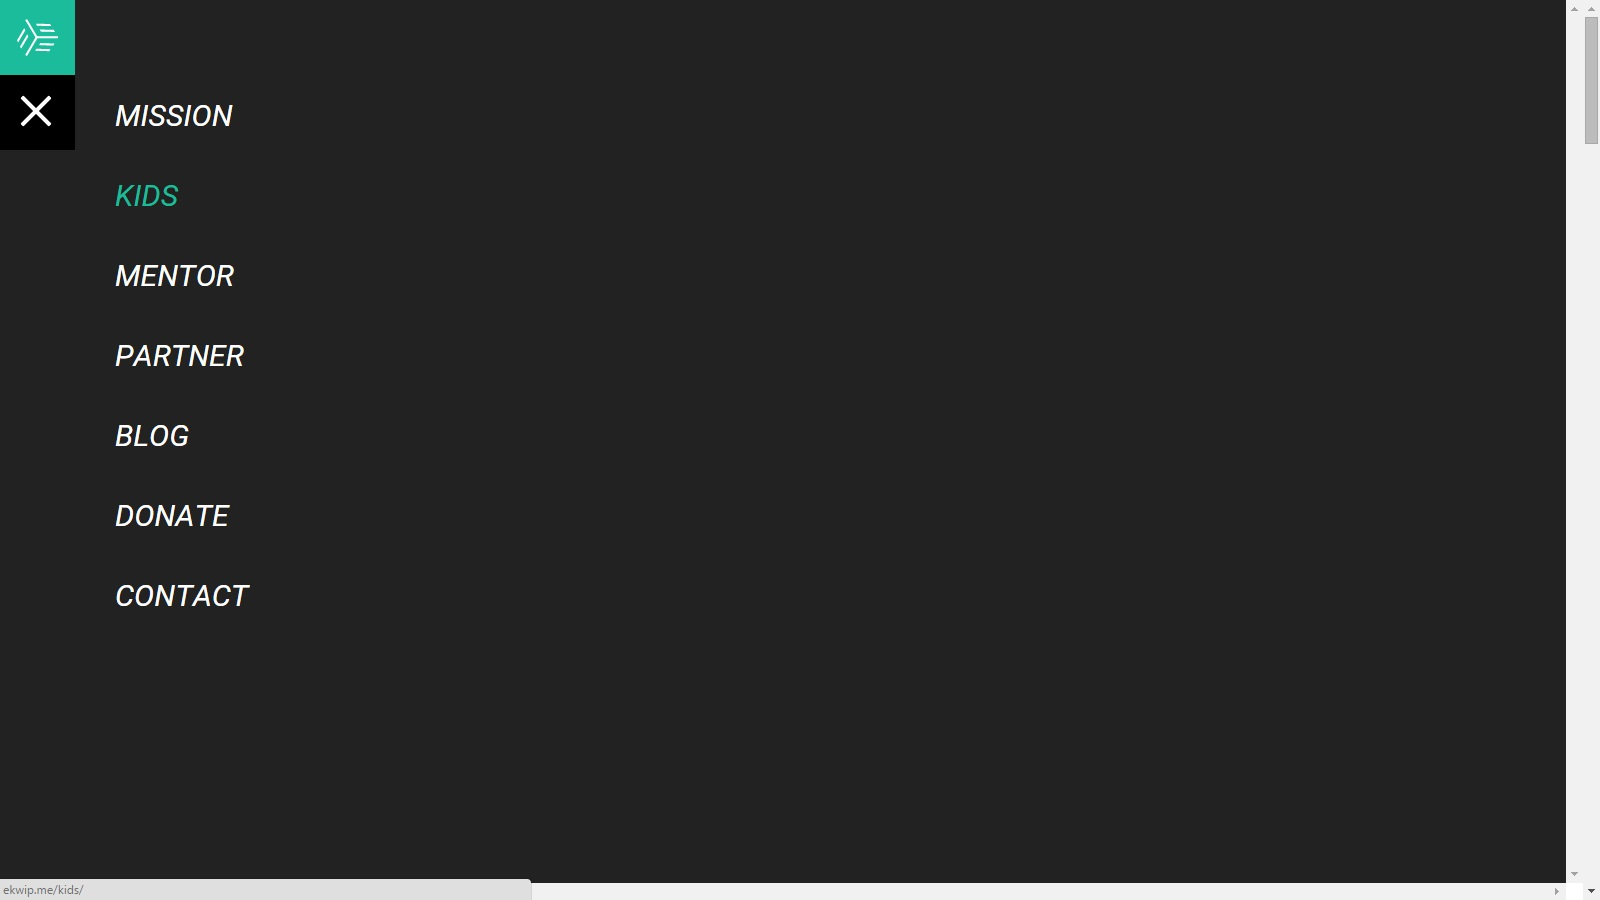
\includegraphics[width=0.45\textwidth]{figuras/refmenu.jpg}\label{primbasefotos:1}}
  \hfill
  \subfloat[imagem de referência - frame]{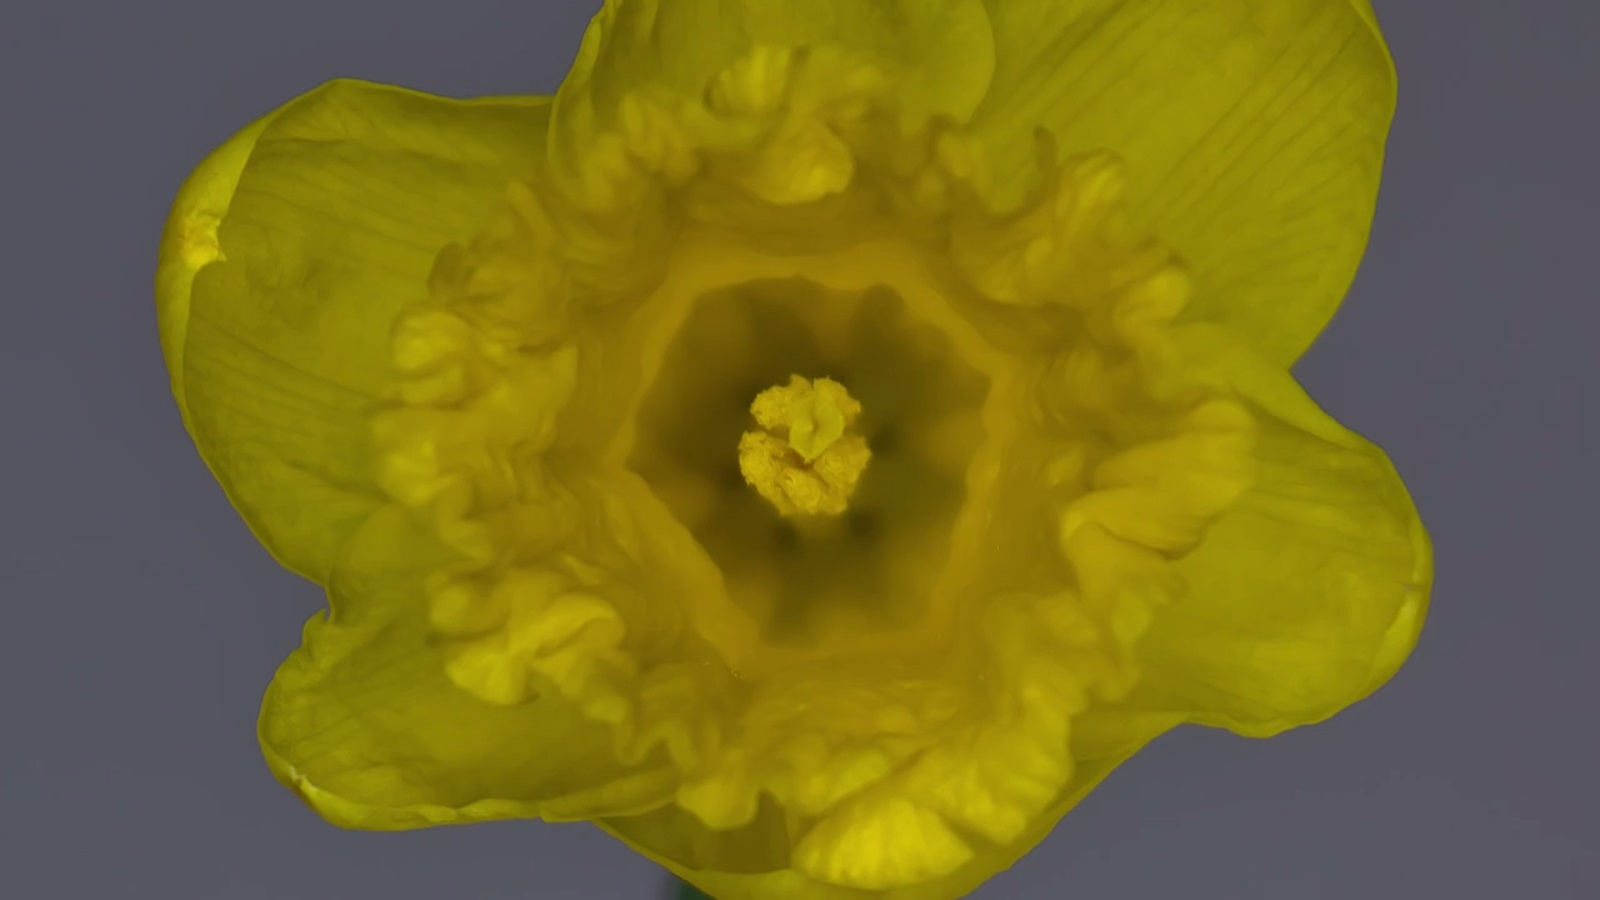
\includegraphics[width=0.45\textwidth]{figuras/refvid.jpg}\label{primbasefotos:2}}
  \hfill
  \subfloat[foto - menu]{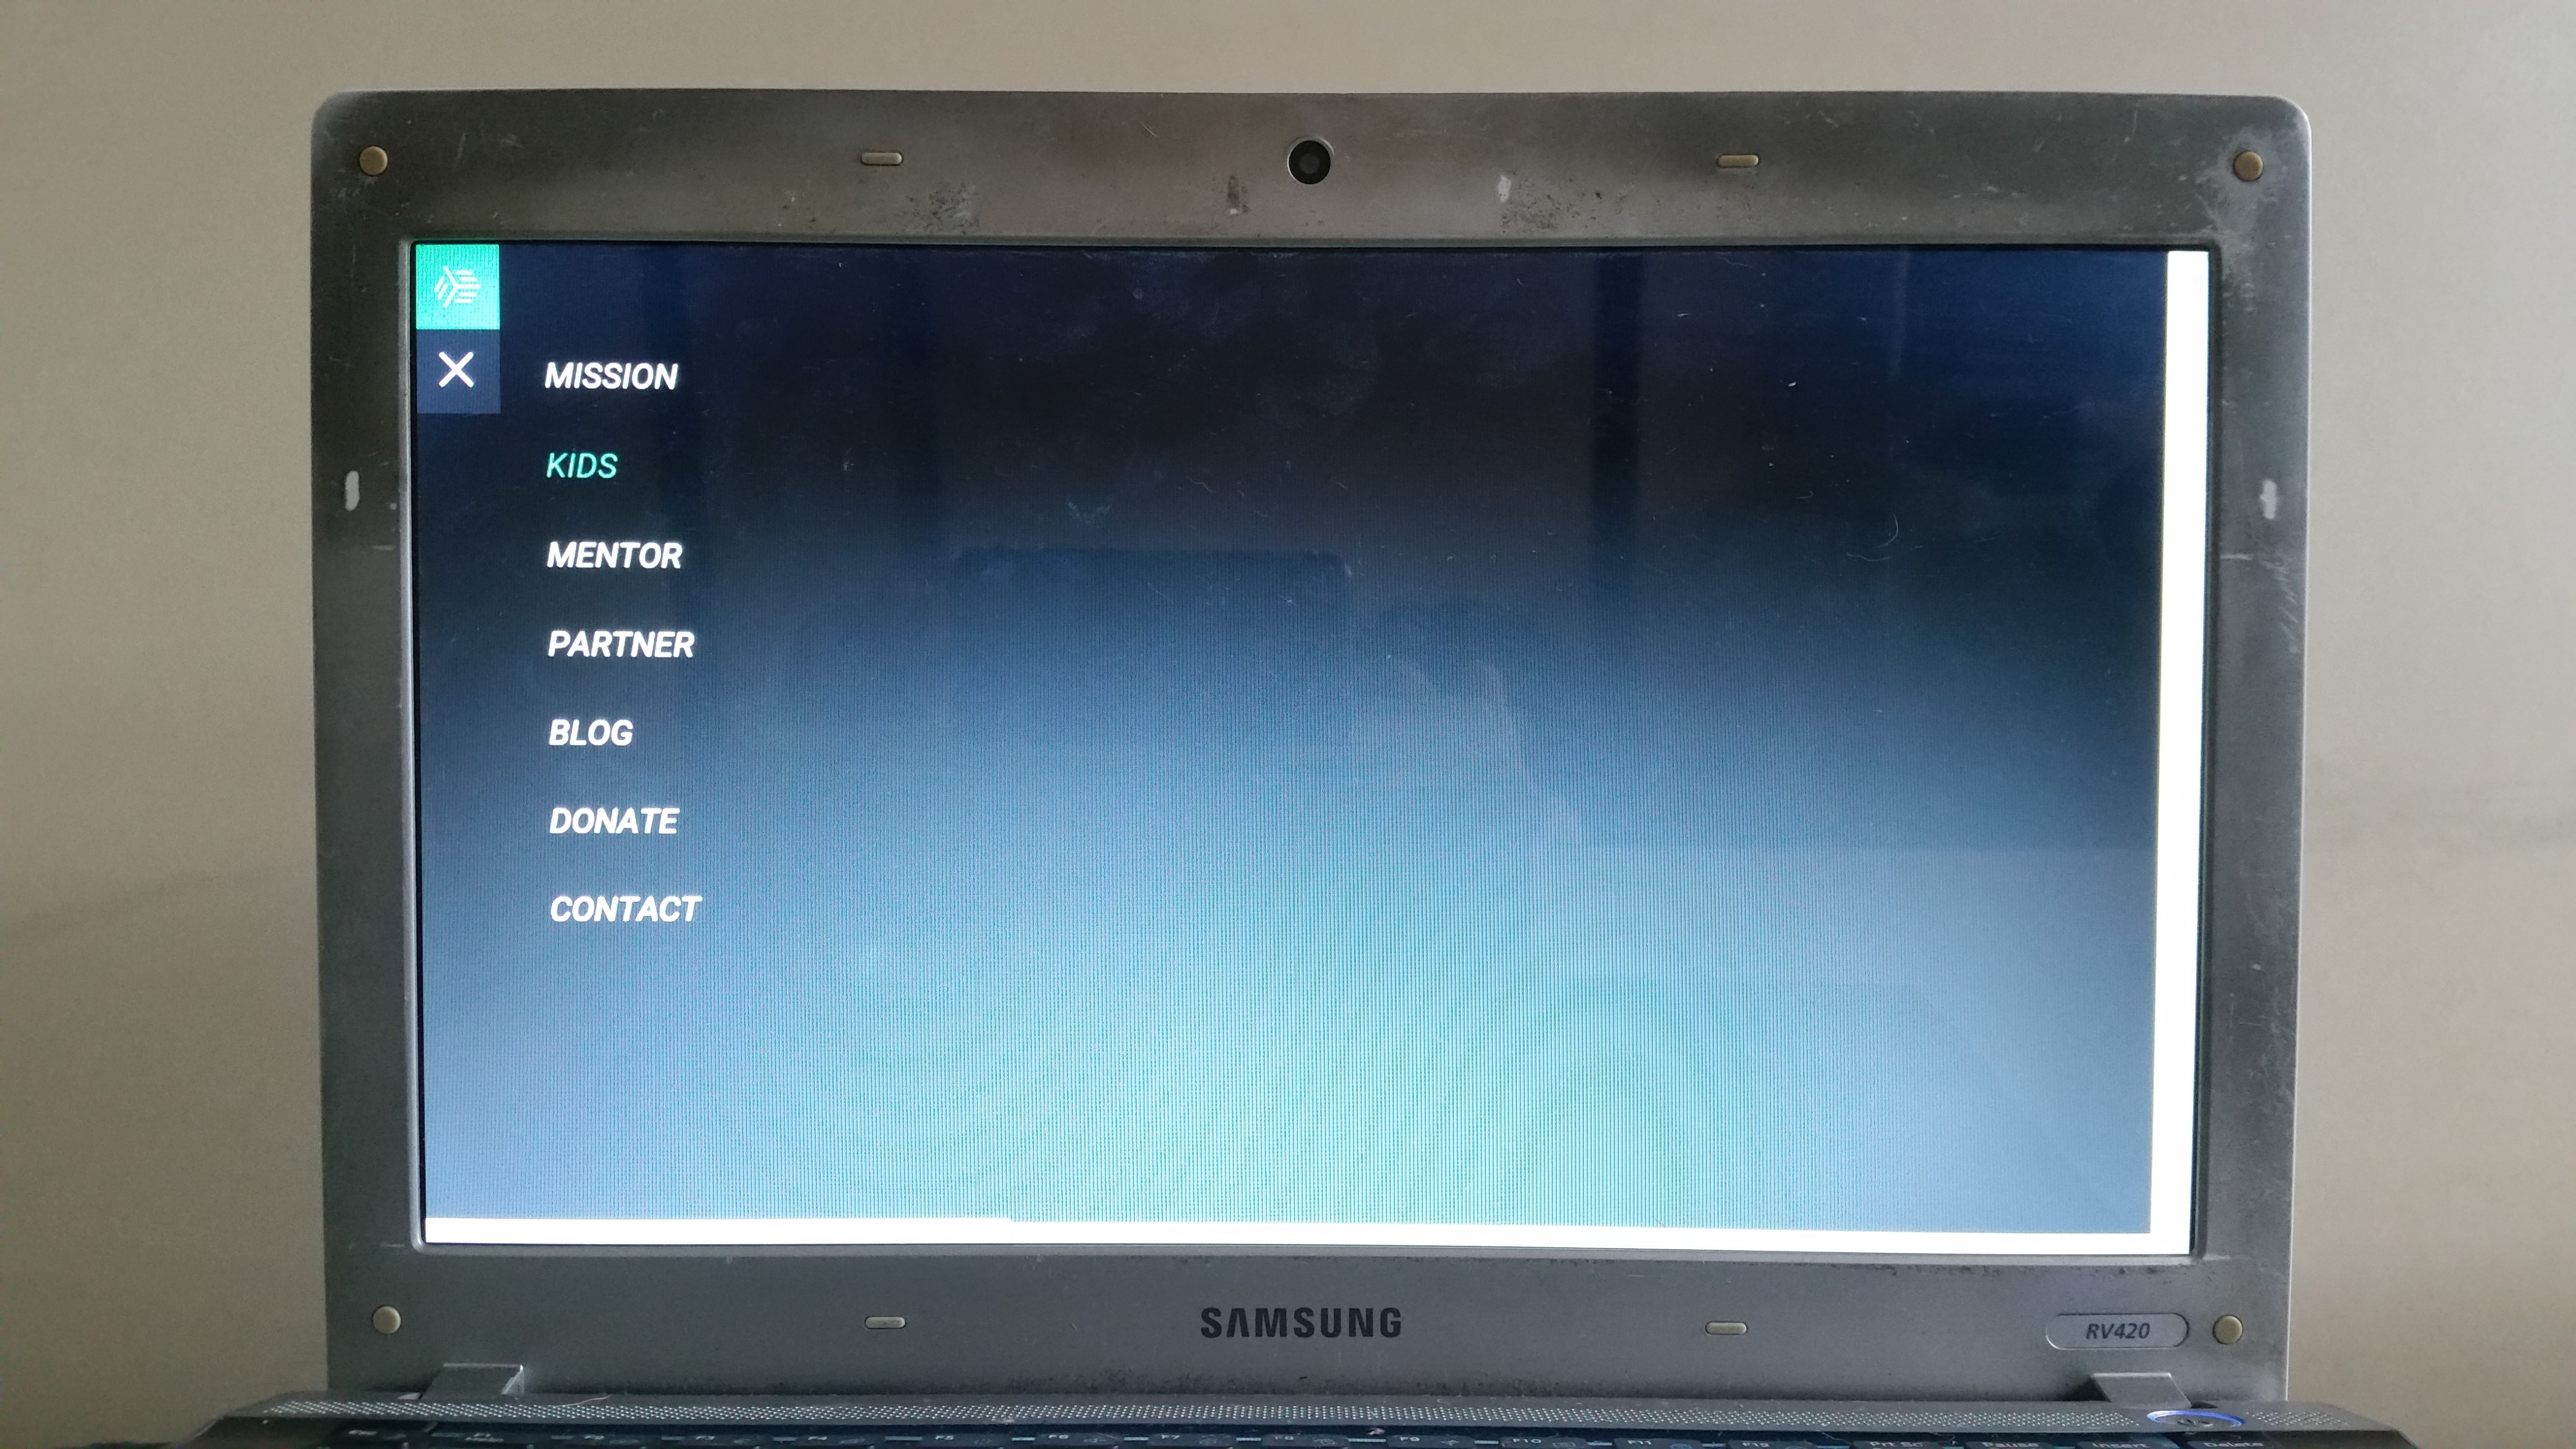
\includegraphics[width=0.45\textwidth]{figuras/fotomenu.jpg}\label{primbasefotos:3}}
  \hfill
  \subfloat[foto - frame]{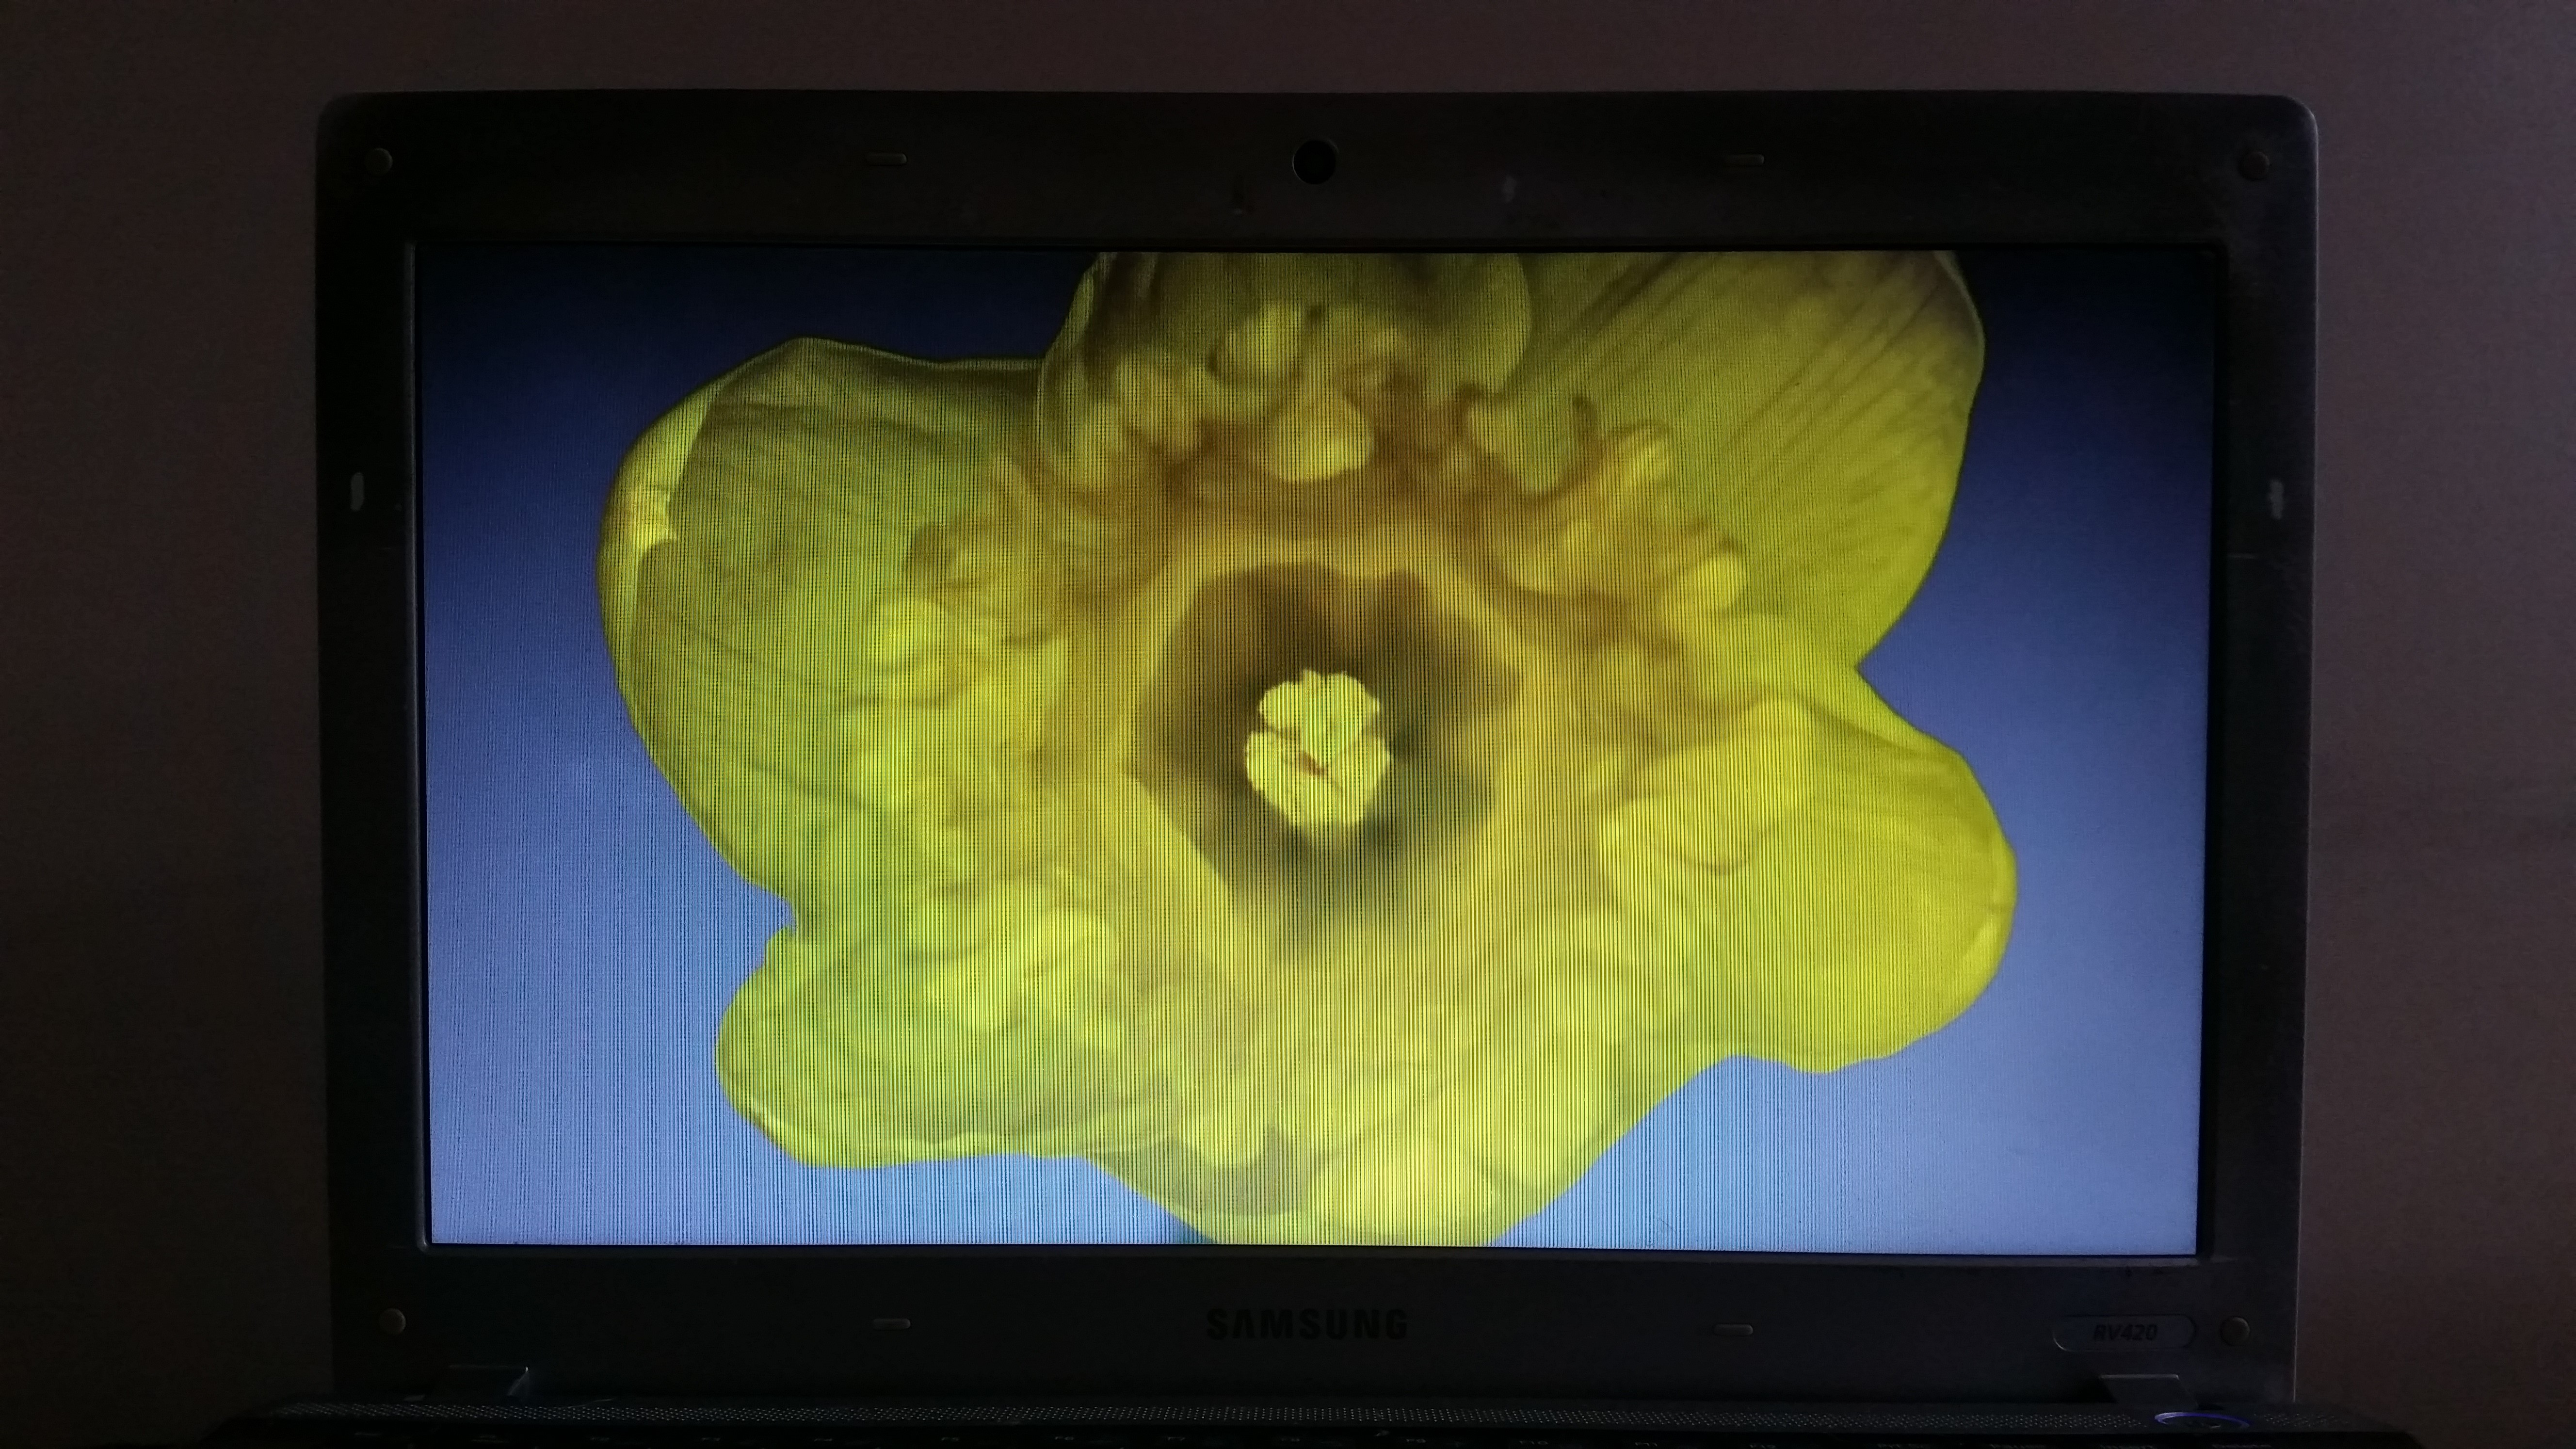
\includegraphics[width=0.45\textwidth]{figuras/fotovid.jpg}\label{primbasefotos:4}}
  \caption{Imagens da primeira base. As figuras \ref{primbasefotos:1} e \ref{primbasefotos:2} mostram imagens de referência e as imagens \ref{primbasefotos:3} e \ref{primbasefotos:4} são fotografias dos	 monitores mostrando os respectivos conteúdos de referência.}
  \label{primbasefotos}
\end{figure}


%Em uma breve descrição geral, na base de dados BioID temos um total de 1521 imagens contendo faces humanas frontais em nível de cinza de 23 indivíduos diferentes. A resolução das imagens é de 384 × 286 pixels. As faces possuem variações de escala (algumas estão perto da câmera e outras não), iluminação e pequenas rotações. Alguns indivíduos usam óculos, outros têm barba e/ou bigode. As imagens desta base de dados possuem rótulos manuais para 20 pontos fiduciais, porém estes rótulos são imprecisos em diversas imagens.


\subsection{Segunda Base}

Para a segunda base, uma câmara escura foi montada a fim de garantir que as fotos teriam o mínimo de interferência externa possível. A câmara foi formada por uma estrutura cúbica, de tamanho suficiente para que os monitores e a câmera pudessem ficar dentro dela, e coberta para não deixar passar luz.

\begin{figure}
 \centering
 \subfloat[estrutura sem cobertura]{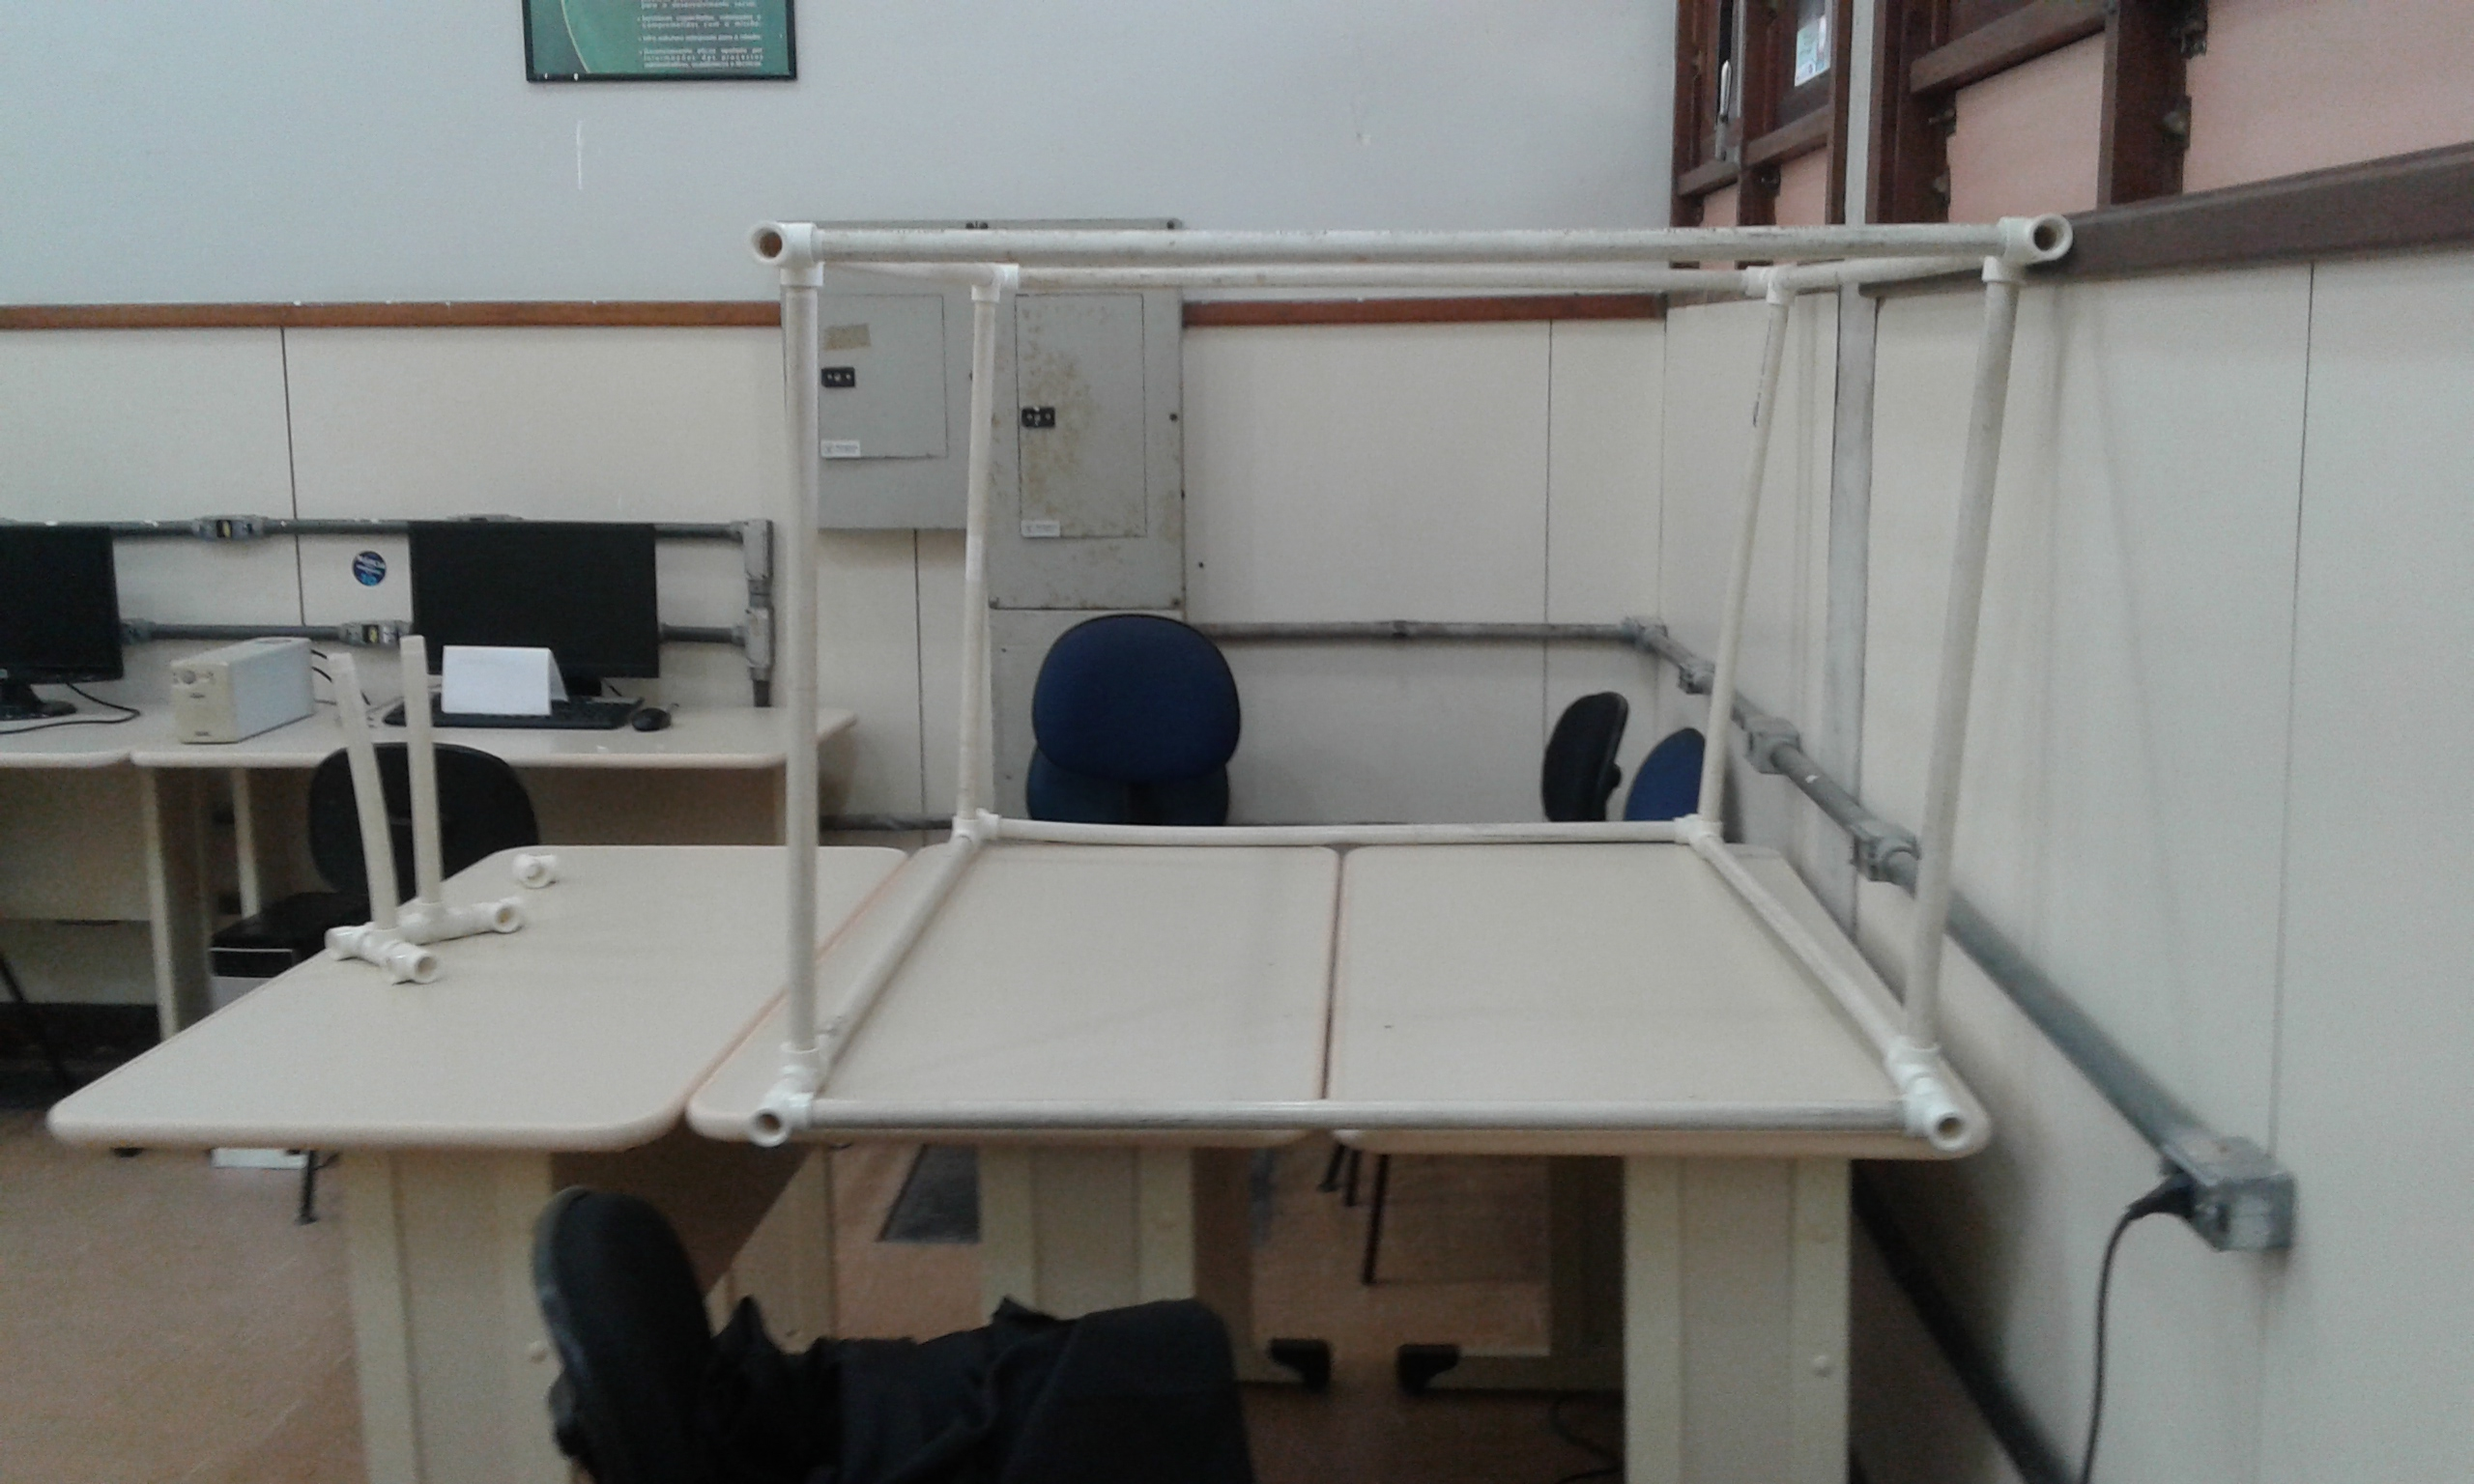
\includegraphics[width=0.45\textwidth]{figuras/camara00.jpg}\label{camaraescura:1}}
  \hfill
  \subfloat[estrutura com cobertura completa]{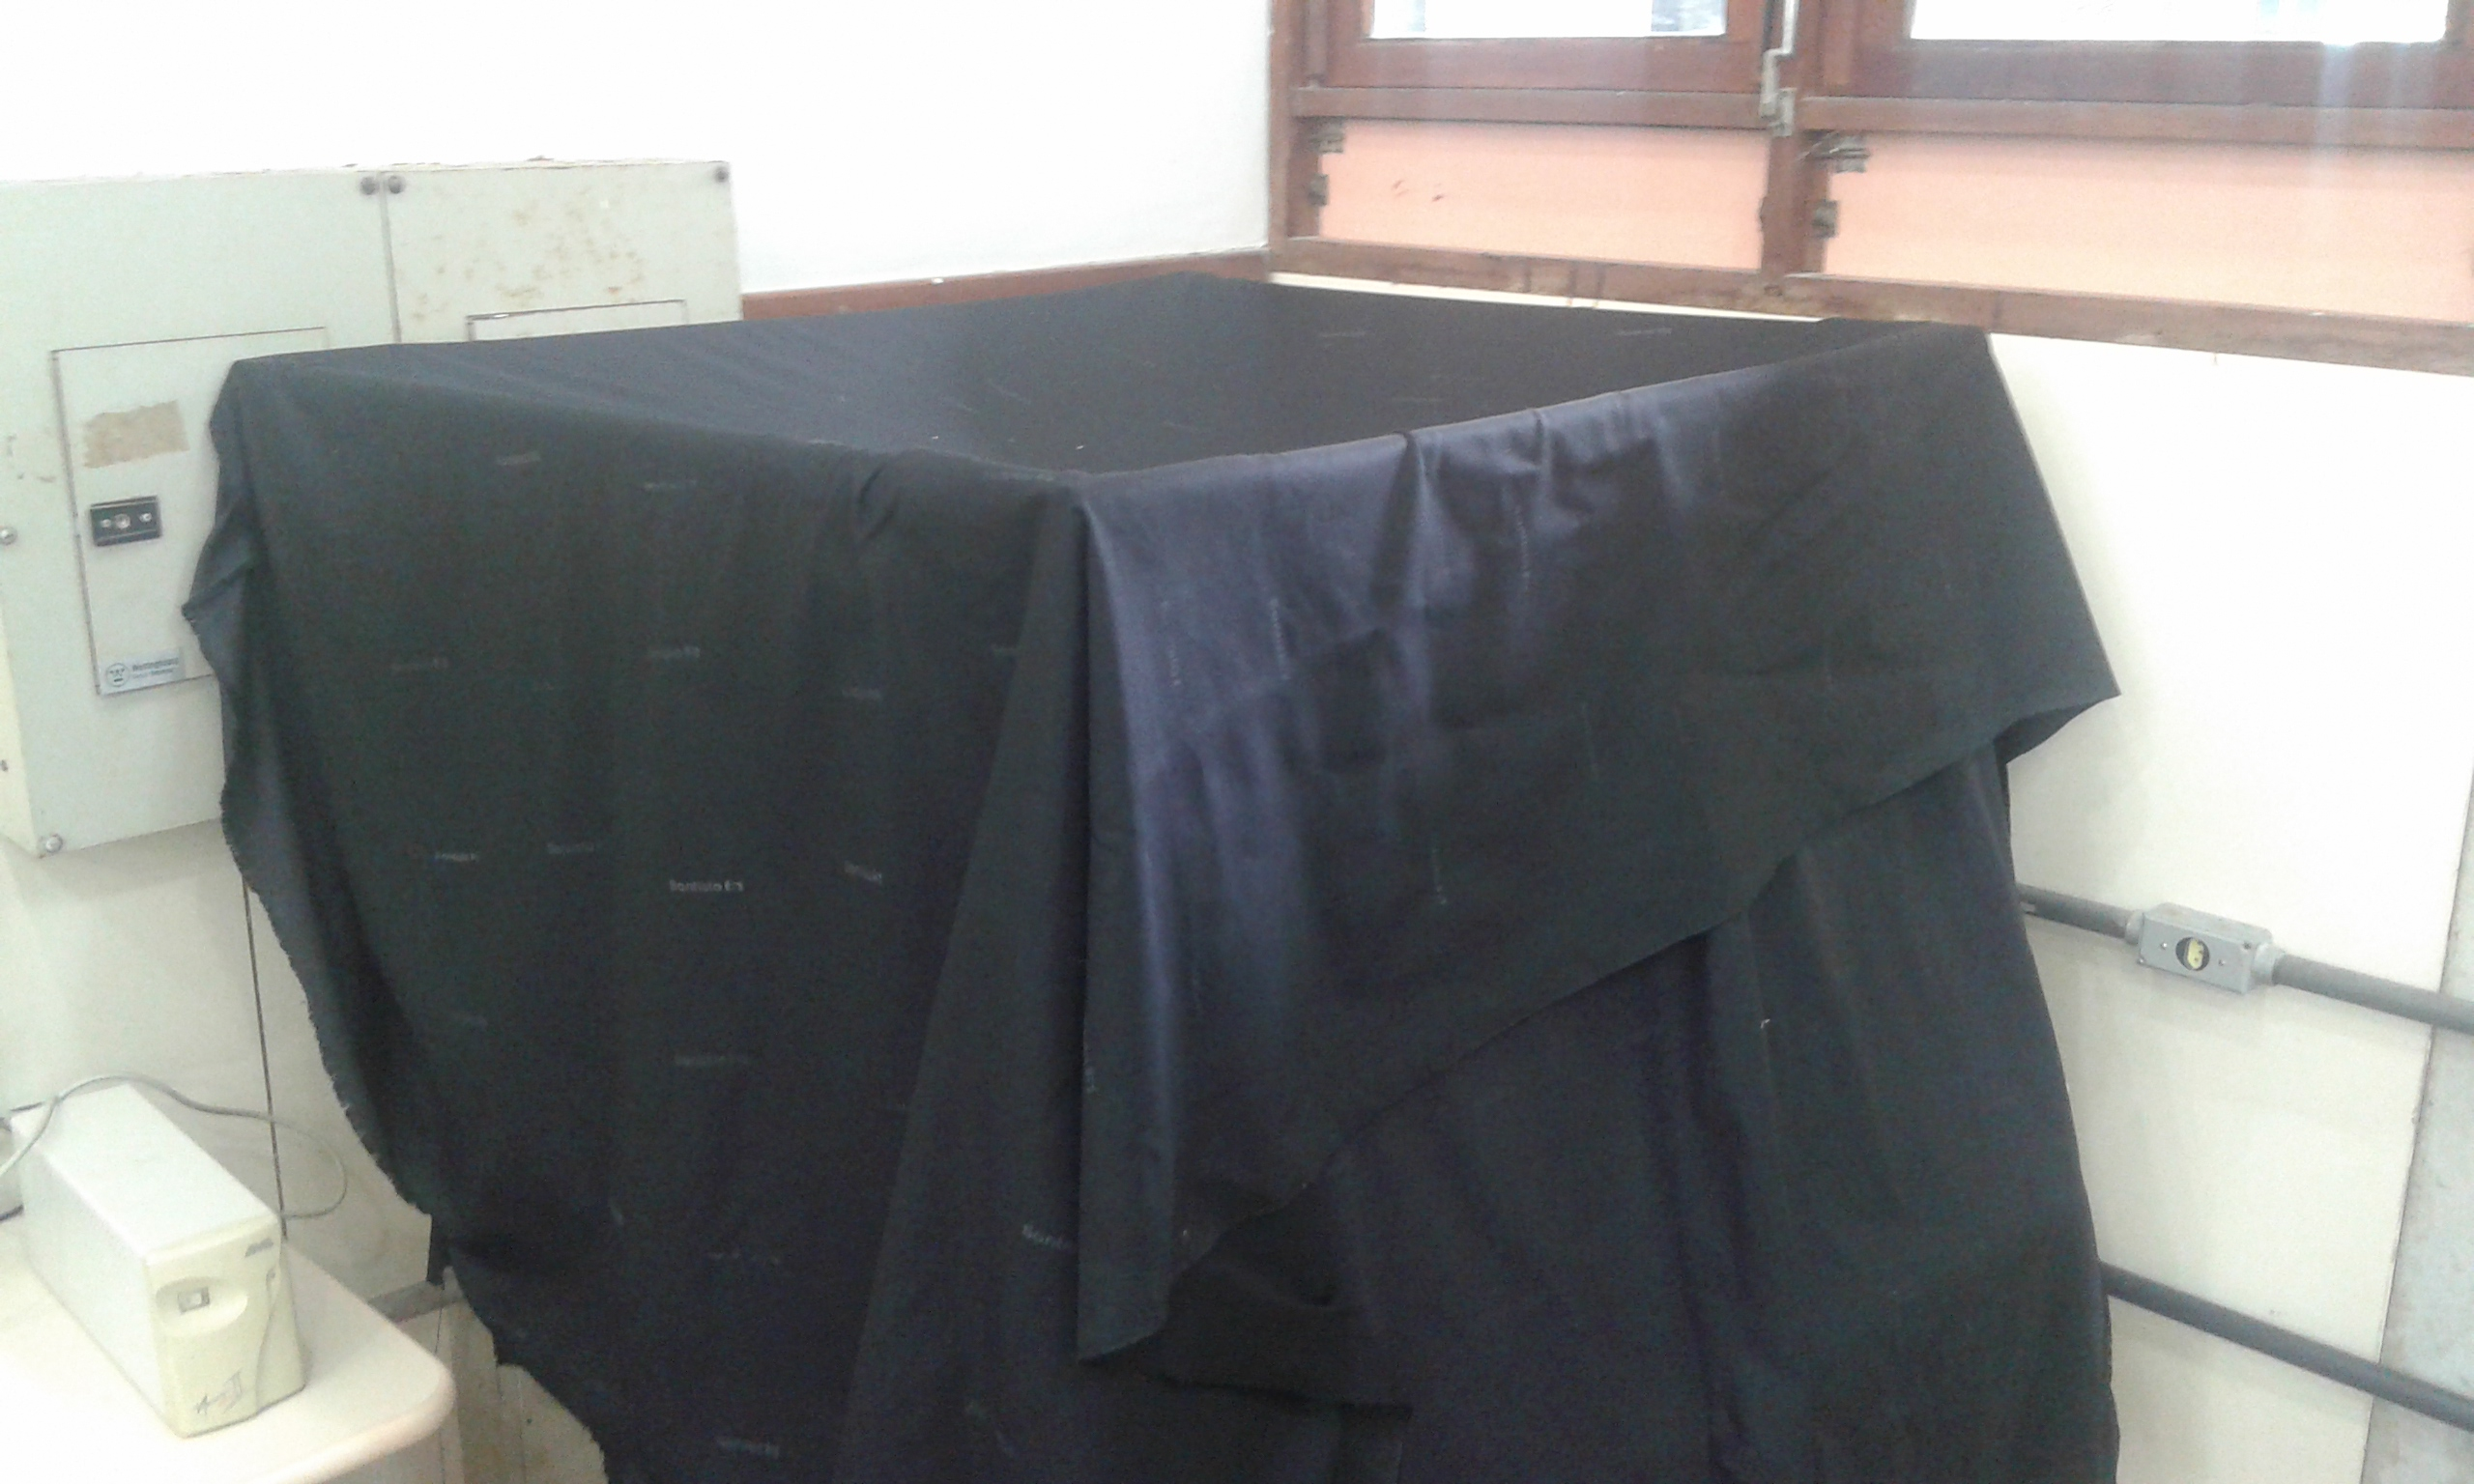
\includegraphics[width=0.45\textwidth]{figuras/camara01.jpg}\label{camaraescura:2}}
  \caption{camara escura.}
  \label{camaraescura}
\end{figure}


%Os monitores e a câmera foram levados para dentro da estrutura. Outra diferença da primeira para a segunda base foi a escolha de mais imagens de referência. Como referência foram utilizadas as seguintes imagens:



Foram escolhidas imagens de referência com uma diversidade maior que na primeira base, de modo que pudessem ser feitos experimentos diferentes e mais específicos nas fotos da segunda base. Como referência foram utilizadas as seguintes imagens:
\begin{itemize}
\item \textbf{um grid} branco de linhas pretas, para poder verificar a eficiência do método quando há muitos objetos retangulares na imagem;
\item \textbf{um xadrez} preto e branco, visando verificar a eficiência do programa com imagens que possuem muitos objetos retangulares de cores diferentes;
\item \textbf{o índio}, figura de referência para testes de TV antigos que ajudava a verificar a qualidade da transmissão da imagem;
\item \textbf{barra de cores} saturada em 20\%, 60\% e 100\%. Estas imagens podem ajudar a analisar como o monitor reage à saturação;
\item \textbf{as três cores primárias puras}, saturadas em em 20\%, 60\% e 100\%, com o mesmo objetivo do colorbar, analisando por cor;
\item \textbf{as três cores secundárias puras}, saturadas em em 20\%, 60\% e 100\%, com o mesmo objetivo das imagens do colorbar e cores primárias;
\item \textbf{12 fotos} de ambientes reais, com o objetivo de analisar a eficiência do método com imagens com alto nível de detalhe;
\item \textbf{4 menus}, visando analisar a eficiência do método em diferenciar opções de menu;
\end{itemize}

Todas as imagens são coloridas e têm tamanho variado. As fotos foram capturadas pela mesma câmera do celular Samsung Galaxy S5 sem flash e todas têm a resolução máxima da câmera, 5312 x 2988 pixeis. Novamente, os monitores foram fotografados ligados e mostrando as imagens de referência. A distância entre a câmera e os monitores é variável. Assim como na primeira base, cada imagem tem um rótulo manual que informa as coordenadas dos quatro pontos que limitam a tela da TV ou monitor.


\section{Métricas de Desempenho} \label{exp:metrica}


\subsection{Primeiro Experimento} \label{exp:metrica1}

%\textcolor{red}{A métrica utilizada aqui é a taxa de detecção}

No primeiro experimento, é encontrado um conjunto de quatro coordenadas que correspondem aos quatro vértices de uma região da imagem. Nosso problema está em classificar a região encontrada como a tela da TV/monitor ou não. Assim, a região encontrada pode pertencer a uma das duas classes mostradas a seguir, tais que:

\begin{equation} \label{eq:class0}
regiao = \begin{cases}
		1, \text{se for tela} \\ 
        0, \text{se não for tela} \\
        \end{cases}
\end{equation}

A imagem é rotulada com quatro coordenadas que correspondem aos pontos que delimitam a tela da TV ou monitor naquela imagem, portanto consideradas o \textit{ground truth}. A classificação é feita calculando a distância entre as coordenadas encontradas pelo método e as coordenadas com que a imagem é rotulada. Esta distância pode ser matematicamente representada através da equação \ref{eq:distpts}:

\begin{equation} \label{eq:distpts}
d_i = \sqrt[]{(gt_i(x)-c_i(x))^2)+(gt_i(y)-c_i(y))^2)}
\end{equation}

Em que $gt_i(x,y)$ é a coordenada do rótulo no $i$-ésimo ponto da imagem, e $c_i(x,y)$  é a coordenada encontrada pelo método que corresponde a $gt_i(x,y)$ e $d_i$ é a distância entre estas duas coordenadas.

O método é considerado correto se todos os pontos encontrados corresponderem aos pontos do \textit{ground truth}, portanto o critério de classificação pode ser matematicamente representado por:

\begin{equation} \label{eq:class1}
regiao = \begin{cases}
		1, \text{se } d_i < \alpha*max(lin,col), \forall i \\ 
        0, \text{se } d_i \geq \alpha*max(lin,col), \forall i \\
        \end{cases}
\end{equation}

Em que $lin$ corresponde ao comprimento do retângulo encontrado, $col$ corresponde à largura e $\alpha$ corresponde a uma constante que indica a tolerância para indicar se o método conseguiu ou não representar a tela da TV.

\subsection{Segundo Experimento}

%\textcolor{red}{A métrica utilizada aqui é a correta identificação das imagens/fotos}

Nestes experimentos, o desempenho do sistema é medido através da sua capacidade de corretamente diferenciar imagens. Esta capacidade é aferida através de três técnicas que comparam a imagem encontrada pelo método com uma ou mais imagens de referência. Estas técnicas são mostradas a seguir:

\begin{itemize}
\item LAE (Least Average Error)
\end{itemize}

%LAE

O método LAE divide a imagem de teste e a de referência em regiões consideradas atômicas. Ele compara cada região na imagem de teste com a região correspondente na imagem de referência, portanto necessitando que as duas imagens tenham o mesmo tamanho e formato. Diferenças na iluminação entre as imagens comparadas podem resultar em valores de intensidade diferentes para a imagem, mesmo representando o mesmo objeto ou a mesma região. A fim de reduzir esta diferença, primeiramente as imagens são normalizadas utilizando a normalização estatística padrão. Dada uma imagem $A$, sua média $\mu_A$ e seu desvio padrão $\sigma_A$ são calculados e a imagem normalizada $A_n$ é dada pela equação \ref{normal}:

\begin{equation}
A_n = \frac{A-\mu_A}{\sigma_A} \label{normal}
\end{equation}

Assim, a média e o desvio padrão são calculados pixel a pixel para cada um dos três canais da imagem (R, G e B) e suas dessimilaridades são computadas e acumuladas, segundo a equação \ref{lae}:

\begin{equation}
D = \sum_ {x,y}^{} \sum_{c=R,G,B}^{} \left | \frac{A(x,y)-\mu _A}{\sigma _A} - \frac{B(x,y)-\mu _B}{\sigma _B} \right |
\label{lae}
\end{equation}

\begin{itemize}
\item NCC (Normalized Cross-Correlation)
\end{itemize}

O método NCC é baseado na correlação cruzada para medir a similaridade entre duas imagens. Assim como no LAE, para diminuir erros devido à diferença de iluminação, primeiramente as imagens são submetidas à normalização estatística padrão. A similaridade entre imagens normalizadas $A_n$ e $B_n$ é calculada segundo a equação \ref{ncc1}:

\begin{equation}
S = \iint A_n(x,y)*B_n(x,y) dx dy \label{ncc1} 
\end{equation}

ou, na forma discreta:

\begin{equation}
S = \sum \sum A_n(x,y)B_n(x,y) \label{ncc2} 
\end{equation} 


Sendo uma imagem normalizada segundo a equação:

\begin{equation}
A_n = \frac {A(x,y) - \mu_A}{\sqrt {\frac{1}{N}(\sum \sum {A(x,y)-\mu_A})^2}} \label{ncc3} 
\end{equation} 

em que $N$ é o número de pixels da imagem $A$, podemos calcular a similaridade entre duas imagens $A$ e $B$ segundo a equação \ref{ncc4}:

\begin{equation}
S = \frac{\sum \sum (A(x,y)-\mu _A)(B(x,y)-\mu _B)}{\sqrt{\sum \sum (A(x,y)-\mu _A)^2}\sqrt{\sum \sum (B(x,y)-\mu _B)^2}}
\label{ncc4}
\end{equation}

\begin{itemize}
\item NCC-BB (Normalized Cross-Correlation using Blocks)
\end{itemize}

Este método foi criado para contornar um problema encontrado pelo método NCC: sua pontuação depende do conteúdo da imagem, portanto tornando difícil a tarefa de escolher um limiar de similaridade que respondesse bem a qualquer imagem. Nele, é calculada a similaridade relativa entre as imagens.
Para isto são executados os seguintes passos:
\begin{itemize}
\item As imagens a ser comparadas são divididas em um $n$ blocos menores de mesmo tamanho;
\item É calculada a correlação cruzada da imagem de referência com uma imagem considerada correta para cada um dos blocos. Estes valores de similaridade são então guardados como um conjunto de valores padrão $S_{padrao}$;
\item Para cada imagem de teste submetida ao método, é calculada a correlação cruzada em cada um dos seus blocos;
\item Os valores de similaridade encontrados são comparados bloco a bloco e somados para compor o valor de similaridade relativa. Sendo $S_{A,B}$ a similaridade entre as imagens $A$ e $B$, a similaridade relativa pode ser calculada através da equação \ref{nccbb}

\begin{equation}
S = \max_{blocos}|S_{A,B} - S_{padrao}| \label{nccbb}
\end{equation}

\end{itemize}

Em cada um dos experimentos, são calculadas as pontuações para cada imagem testada em relação às imagens de referência. Estas pontuações são usadas como critério de avaliação para determinar a qual classe a imagem pertence. 

%era bom colocar um exemplo aqui né....

Por exemplo, na Figura \textbf{insere figura amigão. uma imagem de teste, duas de referência} \textbf{a} temos uma foto da base de dados que é comparada com as imagens \textbf{b} e \textbf{c}. Suas pontuações em cada um dos métodos é dada na tabela \textbf{insere tabela man}.

Imagens cuja pontuação reflete corretamente a que classe elas pertencem são consideradas um corretas. As imagens cuja pontuação não indica corretamente a que classe pertencem são consideradas erradas???


\section{Procedimentos}

\subsection{Pré-processamento} \label{exp:prep}

%REDIMENSIONAMENTO(POUCA COISA MAS TEM): http://www.ipol.im/pub/art/2012/gjmr-lsd/article.pdf

Todos os experimentos tiveram os mesmos procedimentos de pré-processamento. A Figura \ref{fig:diagpreproc} mostra o diagrama de blocos dos procedimentos de pré-processamento utilizados. A primeira etapa é a de redimensionamento da imagem para uma dimensão pré-definida. Após isto é feita a correcão de gama e, por fim, é feita a filtragem gaussiana.

\begin{figure} [h]
\centering
	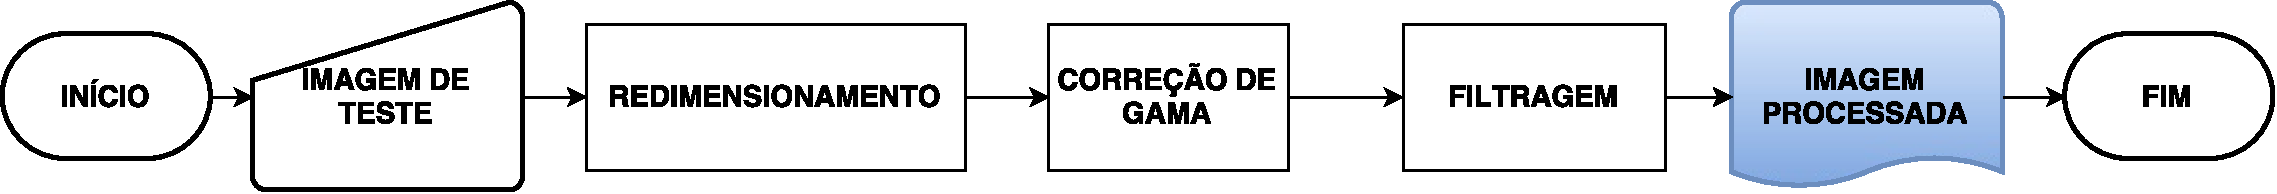
\includegraphics[width = \textwidth]{figuras/preproc.pdf} \label{fig:diagpreproc} \caption{Esquema de pré-processamento utilizado nos experimentos.}
\end{figure}

%redimensionamento
A imagem é redimensionada através de interpolação linear para um tamanho pré-definido, a fim de diminuir o tempo de processamento e uso de recursos. O tamanho escolhido foi 640 $x$ 480.

%correção de gama
%A correção de gama é um método de pré-processamento muito utilizado na literatura \textbf{fontes amigão}. Ela 

A correção de gama é uma transformação dos valores de intensidade da imagem. É uma transformação que tem como objetivo ajustar a luminância da imagem, levando em conta a relação não-linear entre o valor do pixel e a intensidade mostrada. A literatura apresenta exemplos da utilidade da correção de gama para obter melhores imagens de borda \cite{corrgamma00,corrgamma01}.

A transformação é dada pela equação \ref{eq:corrgamma}:

\begin{equation}
I_{corrigida} = {I_{não corrigida}}^\gamma
\label{eq:corrgamma}
\end{equation}

Em que $\gamma$ tem valores acima de zero. Caso $\gamma >1$, os valores de intensidade são comprimidos de forma não-linear, destacando as intensidades mais altas. Com $\gamma <1$ os valores são expandidos, destacando as intensidades mais escuras.

%filtragem gaussiana

%filtro gaussiano, unsharp e depois gaussiano
O último estágio de pré-processamento é a filtragem gaussiana. Este procedimento está ligado ao primeiro procedimento do método, que é a detecção de bordas. O processo de filtragem através do filtro gaussiano tem como objetivo atenuar ruído na imagem, a fim de que as bordas sejam acentuadas mas não o ruído \cite{canny,borda00}.

\subsection{Primeiro Experimento} \label{exp:proc1}

Na Figura \ref{fig:exp1} mostramos o diagrama de blocos do primeiro experimento. O procedimento para uma imagem é mostrado. Primeiramente, efetuamos os procedimentos de pré-processamento, conforme explicados na subseção \ref{exp:prep}. Após isto, o procedimento de extração do retângulo que representa a tela é iniciado. Ele é explicado no Capítulo \ref{met}. A detecção de bordas é executada como explicado na seção \ref{met:borda}. A informação de borda é utilizada no processo de detecção de linhas, conforme visto na seção \ref{met:linha}. O reconhecimento de retângulos e a escolha do retângulo que representa a tela são, então, executados. Os procedimentos são como mostrado em \ref{met:retangulo}. O resultado desta etapa é um conjunto de coordenadas que representa o retângulo encontrado. Estas coordenadas são comparadas com as coordenadas com as quais a imagem é rotulada, como mostrado na subseção \ref{exp:metrica1}. Sua distância é computada e utilizada para classificar a imagem.

\begin{figure} [h]
\centering
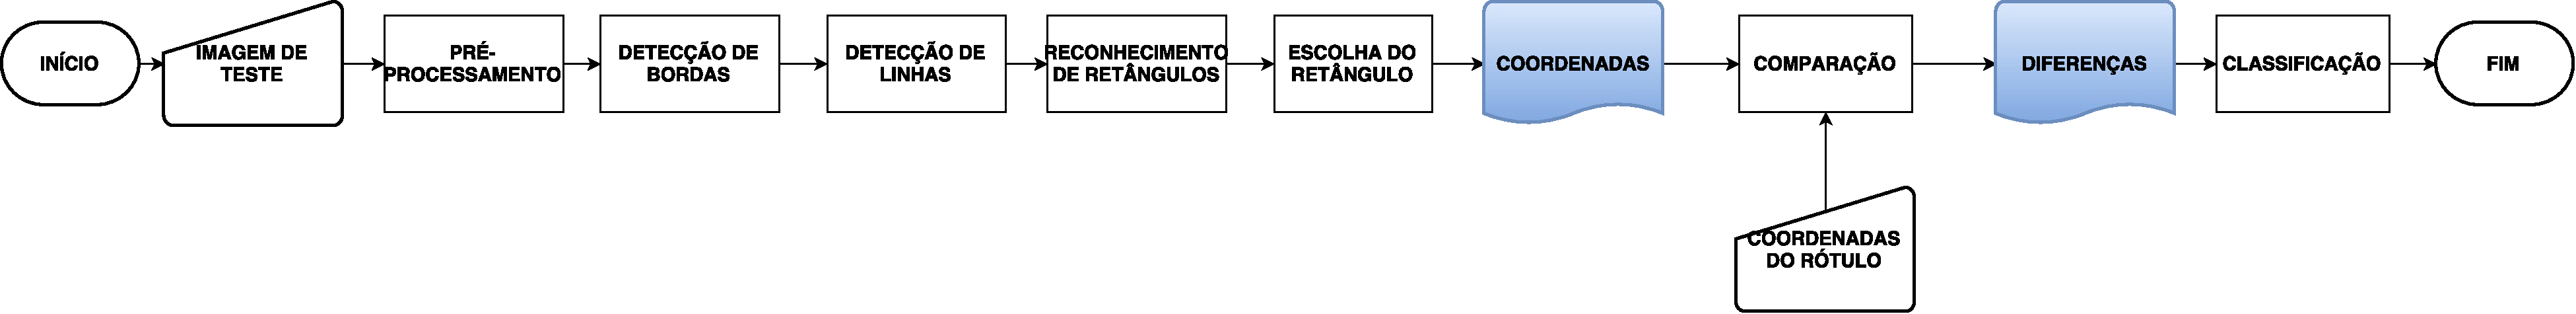
\includegraphics[width = \textwidth]{figuras/exp1.pdf} \label{fig:exp1} \caption{Outline dos primeiros experimentos.}
\end{figure} 


\subsection{Segundo Experimento} \label{exp:proc2}

Na Figura \ref{figexp2} mostramos o diagrama de blocos que relatam os procedimentos comuns à segunda família de experimentos. A diferença entre os diferentes experimentos da segunda família são as imagens utilizadas como entrada.

Os procedimentos para uma imagem são mostrados. À semelhança dos experimentos mostrados em \ref{exp:proc1}, primeiro são feitos os procedimentos de pré-processamento, conforme explicados na subseção \ref{exp:prep}. Após isto, o procedimento de extração do retângulo que representa a tela é iniciado. Ele é explicado no Capítulo \ref{met}. A detecção de bordas é executada como explicado na seção \ref{met:borda}. A informação de borda é utilizada no processo de detecção de linhas, conforme visto na seção \ref{met:linha}. O reconhecimento de retângulos e a escolha do retângulo que representa a tela são, então, executados. Os procedimentos são como mostrado em \ref{met:retangulo}. Ao contrário dos experimentos mostrados em \ref{exp:proc1}, esta fase dá como resultado uma imagem que contém o conteúdo da tela extraído da imagem original. Esta imagem é comparada com uma ou mais imagens de referência, dependendo do experimento, através das métricas mostradas na subseção \ref{exp:metrica2}. Estas pontuações são computadas e utilizadas para classificar a imagem testada. 

\begin{figure} [h]
\centering
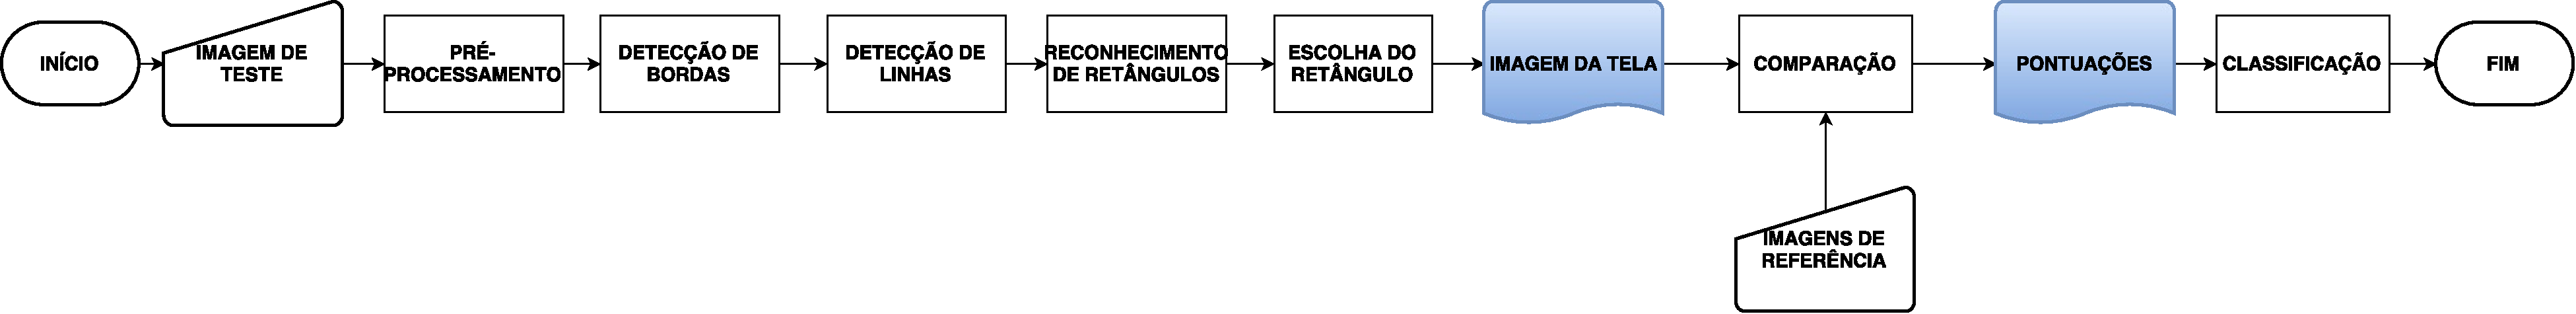
\includegraphics[width = \textwidth]{figuras/exp2.pdf} \label{figexp2}
\caption{Outline dos experimentos.}
\end{figure} 

%procedimentos

\begin{comment}
% introdução

Experimento que aplica o método 

%base de dados

as bases de dados utilizadas no experimento foram a base 1 e a base 2

%métrica de desempenho

As métricas de desempenho foram a similaridade/dessimilaridade medidas com os métodos LAE, NCC e NCC-BB (como mostrado na seção 4.3.5). Testes feitos:
primeira base: 
identificar seleção do menu
diferenciar menu de trecho de vídeo
identificar trechos de vídeo
segunda base:
diferenciar fotos
identificar cores
diferenciar saturação
cores
colorbar
diferenciar cores de fotos
identificar menu


%procedimentos

preprocessamento
sem??
processamento
extração de tela
pos processamento
comparação

%o Testes Feitos entra aqui ou na métrica de desempenho

%resultados
%%os resultados serão expostos assim
%%tabelas/gráficos
%%análise resultados

\subsection{Terceiro Experimento}

% introdução

O experimento aplica o método modificado..




%procedimentos

preprocessamento
correcao gama
redimensionamento
processamento
extração de tela
pos processamento
comparação


\end{comment}

\section{Resultados Experimentais}

%influencia do [INSIRA AQUI MODIFICAÇÃO](resultados)
%%os resultados serao expostos assim
%%tabelas/gráficos
%%análise resultados

\begin{comment}

%EXPERIMENTO PERDIDO PQ AO QUE PARECE É INÚTIL

A figura \ref{fig:exptempo} mostra o diagrama de blocos do funcionamento do primeiro experimento.


\begin{figure} [h]
\centering
	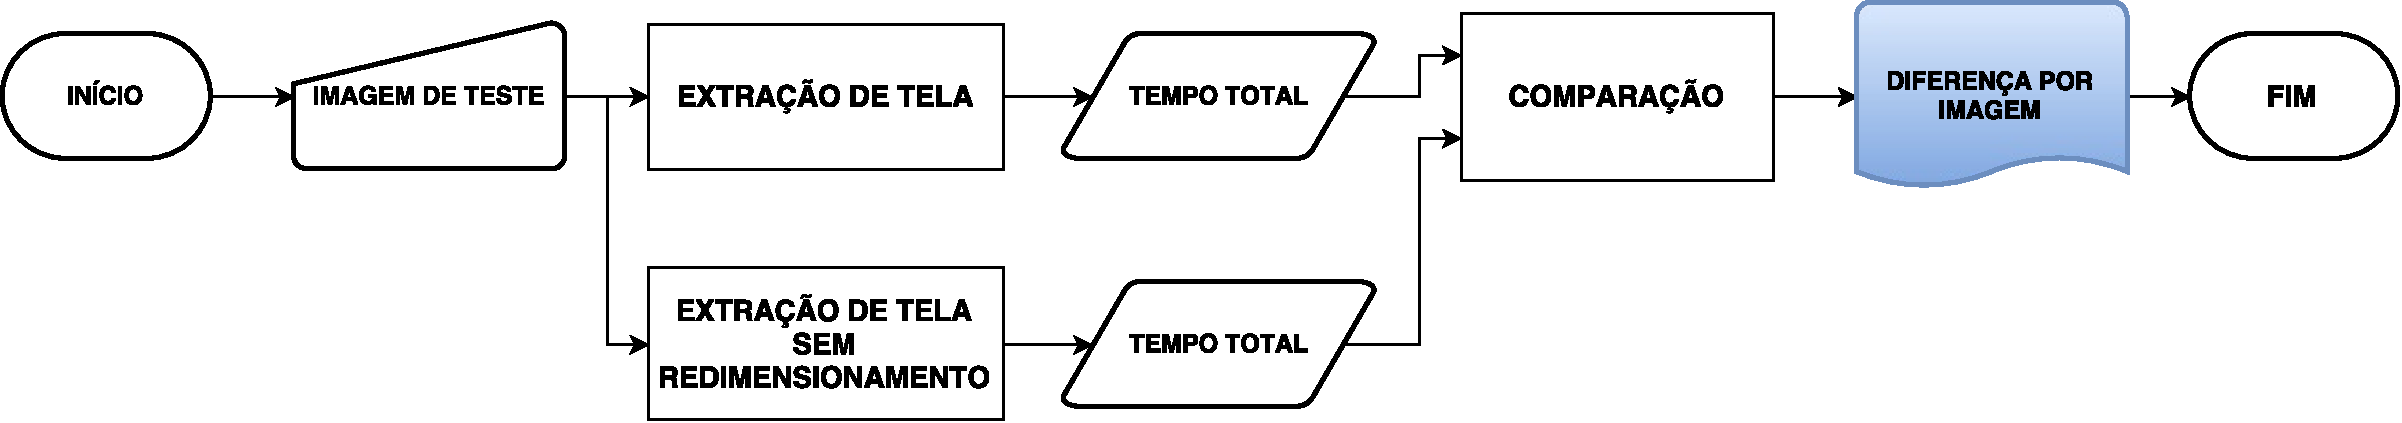
\includegraphics[width = \textwidth]{figuras/experimento_tempo.pdf} \label{fig:exptempo} \caption{Outline do primeiro experimento.}
\end{figure} 

\begin{comment}
% introdução

O experimento apresentado nesta seção foi feitos implementando o método de extração de tela de TV nas mesmas imagens duas vezes, uma com e outra sem redimensionamento.

%base de dados

As imagens escolhidas para compor o conjunto de teste deste experimento foram um subconjunto de 50 imagens aleatoriamente selecionadas da base de dados 1. As imagens são coloridas e têm resoluções 5312 x 2988, [] e [].

%métrica de desempenho

A métrica de desempenho é o tempo utilizado pelo algoritmo para encontrar uma tela de TV.
%Somente telas encontradas contam? fazer mais de um teste? porque? (se não, explicar o porque tbm)
O tempo total utilizado pelas 50 telas é obtido e depois sua média calculada.
%\end{comment}

%procedimentos

%escolha das imagens	aleatorio etc
%preprocessamento correção de gama (pesquisar literatura) redimensionamento (sim em um experimento e nao em outro)



As duas simulações tiveram etapas de preprocessamento distintas. A correção de gama foi utilizada em ambas, porém o redimensionamento, alvo deste experimento, foi utilizado somente em uma delas.
A correção de gama é uma transformação dos valores de intensidade da imagem. É uma transformação que tem como objetivo ajustar a luminância da imagem, levando em conta a relação não-linear entre o valor do pixel e a intensidade mostrada. A literatura apresenta exemplos da utilidade da correção de gama para obter melhores imagens de borda \cite{corrgamma00,corrgamma01}.

%Najafabadi, M. J. E., & Pourghassem, H. (2011, December). A Novel Method for Improving Edge Detection Using Negative and Gamma Correction Functions. In Intelligent Computation and Bio-Medical Instrumentation (ICBMI), 2011 International Conference on (pp. 60-63). IEEE.

%Liu, M., Ding, Y., Wang, X., & Yan, X. (2009, November). Gamma correction with revised piecewise curve and edge directed error diffusion. In Wireless Communications & Signal Processing, 2009. WCSP 2009. International Conference on (pp. 1-4). IEEE.

A transformação é dada pela equação:

\begin{equation}
I_{corrigida} = {I_{não corrigida}}^\gamma
\end{equation}

Em que $\gamma$ tem valores acima de zero. Caso $\gamma >1$, os valores de intensidade são comprimidos de forma não-linear, destacando as intensidades mais altas. Com $\gamma <1$ os valores são expandidos, destacando as intensidades mais escuras.

%redimensionamento

O redimensionamento das imagens de entrada foi feito através de interpolação linear. Esta técnica considera a imagem como uma matriz e interpola os valores dos pixels primeiro no sentido horizontal e depois no vertical. Ela é melhor explicada no Capítulo \ref{met} na subseção \ref{redim}. % (capitulo quatro. mesma explicação?? acho que sim)
 
%processamento extração do conteudo (método)

Após o preprocessamento, as imagens foram então submetidas ao algoritmo de extração de tela da TV. A primeira simulação submete a imagem à etapa de redimensionamento. Portanto, a imagem é reduzida à resolução de 1280 x 960 através da interpolação linear e a imagem reduzida é submetida à extração de tela. O tamanho original da imagem é guardado para que ao fim o retângulo encontrado seja redimensionado e a tela da imagem original seja extraída. %fórmula mostrando o redimensionamento do retangulo???

A segunda simulação submete ao método as imagens após a correção de gama, rendendo desnecessário o método para redimensionamento do retângulo encontrado.

%pos processamento   calculado tempo total   calculado ganho de tempo (como?)

Nas duas simulações, o tempo gasto pelo algoritmo para processar cada imagem é calculado em segundos. As condições de hardware em ambas as simulações é igual. Devido à possibilidade do algoritmo não encontrar um retângulo considerado o contorno da tela, o tempo é dividido pelo número de imagens de tela encontradas, através da equação:

\begin{equation}
T_{médio} = \frac{T_{total}}{n}
\end{equation}

Em que $T_{total}$ é o tempo total que o algoritmo leva para processar as imagens e $n$ é o número de telas encontradas no fim do processamento.

O procedimento é repetido para a segunda simulação. O tempo $T_{médio}’$ é então calculado e é encontrada a diferença entre os tempos:

\begin{equation}
D_tempo = T_{médio}’ - T_{médio}
\end{equation}

%influencia do redimensionamento(resultados)
%%os resultados serão expostos assim
%%tabelas/gráficos
%%análise resultados


\end{comment}

